\section{计算机的浮点数系统及舍入误差}

\begin{frame}\ft{\secname}

\begin{dingyi}[计算机浮点数$f$]
$$
f = \pm ~w ~\times~ \beta^J, \quad L \le J \le U.
$$
其中
\begin{itemize}
\item 
$\beta ~\rightarrow~ \textcolor{acolor4}{\mbox{基底}}$
\item
$J ~\rightarrow~ \textcolor{acolor4}{\mbox{阶}}$
\item
$w ~\rightarrow~ \textcolor{acolor4}{\mbox{尾数:}}\quad
w ~=~ 0~.~d_1~d_2~\cd ~d_t
$
\begin{itemize}
\item $t~\rightarrow~ \textcolor{acolor4}{\mbox{尾数位数(字长)}}$ \\[0.2cm]
\item $0 \le d_i < \beta: \quad d_i \ne 0 ~\Longrightarrow~  \mbox{规格化浮点数}$
\end{itemize}
\end{itemize}
\end{dingyi}

\end{frame}


\begin{frame}\ft{\secname}

\begin{dingyi}[计算机浮点数系统]
$$
\begin{aligned}
\mathcal{F} = \{0\} \cup 
\{f: &  f = \pm 0.d_1d_2\cd d_t ~\times~ \beta^J,\\
& 0 \le d_i < \beta, \quad d_1 \ne 0,\quad L \le J \le U\}\\[0.2cm] \pause 
& \triangleq
\textcolor{acolor5}{(\beta, ~ t, ~ L, ~U)}
\end{aligned}
$$      
\end{dingyi}
\pause 
\begin{itemize}
\item 机器不同,这四个值就不同。较典型的为$(2, 56, -64, 64)$.
\item
$\mathcal{F}$是一个有限集,包含有
$$2(\beta-1)\beta^{t-1}(U-L+1)+1\mbox{个数}$$ 
\item
这些数对称地分布在区间$[m,M]$和$[-M,-m]$中,其中
$$
m = \beta^{L-1}, \quad M = \beta^U(1-\beta^{-t}).
$$
\end{itemize}

\end{frame}


\begin{frame}\ft{\secname}

对于$(\beta, ~ t, ~ L, ~U) = (2,2,-1,2)$,共包含17个数:
$$
\begin{array}{l}
(0.10\times 2^{-1})_2 = (0.010)_2 = 2^{-2} = 0.25 \\
(0.11\times 2^{-1})_2 = (0.011)_2 = 2^{-2} + 2^{-3} = 0.375\\
(0.10\times 2^{0})_2 = (0.10)_2 = 2^{-1} = 0.5\\
(0.11\times 2^{0})_2 = (0.11)_2 = 2^{-1} + 2^{-2} = 0.75\\
(0.10\times 2^{1})_2 = (1.0)_2 = 1\\
(0.11\times 2^{1})_2 = (1.1)_2 = 1 + 2^{-1} = 1.5\\
(0.10\times 2^{2})_2 = (10)_2 = 2^{1} = 2\\
(0.11\times 2^{2})_2 = (11)_2 = 2^{1} + 1 = 3\\
\end{array}
$$
\pause 
\begin{center}
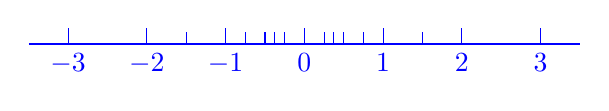
\begin{tikzpicture}
\draw[blue,thick] (-3.5,0)--(3.5,0);
\foreach \x in {-3,-2,-1,0,1,2,3} 
\draw[blue] (\x,0) node[below] {$\x$} -- (\x,0.2);
\foreach \x in {-1.5,-0.75,-0.5,-0.375,-0.25,0.25,0.375,0.5,0.75,1.5} 
\draw[blue] (\x,0) -- (\x,0.15);
\end{tikzpicture}
\end{center}
\pause
由此可看出,这些数的分布是不等距的。

\end{frame}


\begin{frame}\ft{\secname}

$$
\begin{array}{rcl}
\mathcal{F}\mbox{有限}
&\Longrightarrow&
\mathcal{F}\mbox{不可能将}[m,M]\mbox{和}[-M,-m]\mbox{中任意实数精确表示。} \\[0.2cm]
&\Longrightarrow&
\mbox{计算机中浮点数的运算无法精确进行}
\end{array}
$$
\pause 
\begin{li}
\begin{itemize}
\item 数$0.584635$无法用$4$位$10$进制浮点数表示\pause 
\item 两个$t$位浮点数相乘,若要精确一般需要$2t$位,用$t$位浮点数表示自然不精确,由此会产生舍入误差。
\end{itemize}

\end{li}

\end{frame}


\begin{frame}\ft{\secname}

\begin{wenti}
给定一个实数,应选择什么样的浮点数来表示,由此产生的相对误差是多少?
\end{wenti}

\end{frame}


\begin{frame}\ft{\secname} 

\textcolor{acolor5}{浮点数的选取}

记实数$x$的浮点数为$fl(x)$
\begin{itemize}
\item 当$x=0$时,取
$$fl(x) = 0$$
\item 当$m \le |x| \le M$时,取
$$
fl(x) = \left\{
\begin{array}{ll}
\mathcal{F}\mbox{中最接近}x\mbox{的数}f, & \mbox{\textcolor{acolor4}{用舍入法};}\\[0.3cm]
\mathcal{F}\mbox{中满足}|f|\le|x|\mbox{且最接近}x\mbox{的数}f, & \mbox{\textcolor{acolor4}{用截断法}。}
\end{array}
\right.
$$
\end{itemize}

\end{frame}


\begin{frame}\ft{\secname} 
对$(\beta, ~ t, ~ L, ~U) = (10,3,0,2)$
$$
fl(x) = \left\{
\begin{array}{ll}
0.546\times 10, & \mbox{\textcolor{acolor4}{用舍入法}}\\[0.3cm]
0.545\times 10, & \mbox{\textcolor{acolor4}{用截断法}}
\end{array}
\right.
$$

\end{frame}


\begin{frame}\ft{\secname}\fst{实数表示成浮点数的相对误差}

\begin{dingli}
设$m\le |x| \le M$,则
$$
fl(x) = x (1 + \delta), \quad |\delta| \le \epsilon_{machine}
$$
其中$\epsilon_{machine}$为机器精度,即
$$
\epsilon_{machine} = \left\{
\begin{array}{cc}
\frac12 \beta^{1-t}, & \mbox{\textcolor{acolor4}{用舍入法}}\\[0.3cm]
\beta^{1-t}, & \mbox{\textcolor{acolor4}{用截断法}}
\end{array}
\right.
$$
\end{dingli}

\end{frame}


\begin{frame}\ft{\secname}\fst{实数表示成浮点数的相对误差}

\begin{zhengming}
不妨设$x>0$,且设$\alpha$是满足
$$
\beta^{\alpha-1}\le x < \beta^{\alpha}
$$
的唯一整数。
在$[\beta^{\alpha-1}, \beta^{\alpha})$中浮点数的阶为$\alpha$,
所有$t$位浮点数的间距为$\beta^{\alpha-t}$。\pause 
\begin{itemize}
\item    
对于舍入法,因
$$
|fl(x)-x| \le \frac12 \beta^{\alpha-t} 
= \frac12 \beta^{\alpha-1}\beta^{1-t} \le \frac12 x \beta^{1-t} 
$$
故
$$
\frac{|fl(x)-x|}{x} \le \frac12 \beta^{1-t}
$$
\end{itemize}
\end{zhengming}
\end{frame}


\begin{frame}\ft{\secname}\fst{实数表示成浮点数的相对误差}
\begin{proof}
\begin{itemize}
\item    
对于截断法:
$$
|fl(x)-x| \le  \beta^{\alpha-t} 
=  \beta^{\alpha-1}\beta^{1-t} \le  x \beta^{1-t} 
\pause ~~ \Longrightarrow~~
\frac{|fl(x)-x|}{x} \le  \beta^{1-t}
$$
\end{itemize}
\end{proof}

\end{frame}


\begin{frame}\ft{\secname}\fst{基本运算的舍入误差}

设$a, ~b \in \mathcal{F}$为两个给定的浮点数,\textcolor{acolor4}{用$\circ$表示$+,~-,~\times,~/$中的任意一种运算。}
\begin{dingyi}[$fl(a\circ b)$]
先进行运算,得到精确的实数,再按舍入规则表示成浮点数。
\end{dingyi}
\pause
$$
\begin{array}{l}
|a \circ b| > M ~~\rightarrow~~ \mbox{上溢} \\[0.3cm]
0 < |a \circ b| < m ~~\rightarrow~~ \mbox{下溢} 
\end{array}
$$

\end{frame}


\begin{frame}\ft{\secname}\fst{基本运算的舍入误差}

\begin{dingli}
$$
fl(a\circ b) = (a\circ b) (1+\delta), \quad |\delta| \le \epsilon_{machine}
$$
\end{dingli}

\end{frame}


\begin{frame}\ft{\secname}\fst{基本运算的舍入误差}

\begin{li}
设$x, y, z \in \mathcal{F}$,求$fl(x+y+z)$。
\end{li}
\pause
\begin{jie}
$$
\begin{array}{l}
\left.
\begin{array}{l}
fl(x+y+z) = fl(fl(x+y)+z) \\[0.2cm] \pause 
fl(x+y) = (x+y)(1+\delta_1), \quad |\delta_1| \le \epsilon_{machine} 
\end{array}\pause 
\right\}\Longrightarrow \\[0.3in]
\pause 
\begin{array}{rcl}
  fl(x+y+z) &=& fl((x+y)(1+\delta_1)+z) \\[0.2cm]
&=& ((x+y)(1+\delta_1)+z)(1+\delta_2) \\[0.2cm]
&=& (x+y)(1+\delta_1)(1+\delta_2)+z(1+\delta_2)
\end{array}
\end{array}     
$$
\end{jie}

\end{frame}


\begin{frame}\ft{\secname}

\begin{li}
给定$x, y \in \R^n$,估计$|fl(x^Ty) - x^Ty|$的上界。
\end{li}
\pause
\begin{jie}
令$S_k = fl\left(\sum_{i=1}^k x_i y_i\right)$,则
$$
\begin{array}{rl}
S_1 &= x_1y_1(1+\gamma_1), \quad |\gamma_1| \le \epsilon_{machine}, \\[0.2cm]
S_k &= fl(S_{k-1} + fl(x_ky_k)) \\[0.2cm]
&= [S_{k-1} + x_k y_k (1+\gamma_k)](1+\delta_k), \quad |\delta_k|, |\gamma_k| \le \epsilon_{machine}, \\[0.2cm]
\Longrightarrow~& \ds
fl(x^Ty) = S_n = \sum_{i=1}^n x_iy_i\textcolor{acolor5}{(1+\gamma_i)\Pi_{j=i}^n(1+\delta_j)}
= \sum_{i=1}^n\textcolor{acolor5}{(1+\epsilon_i)}x_iy_i    \\[0.2cm]
\Longrightarrow~& \ds
|fl(x^Ty)-x^Ty| \le \sum_{i=1}^n |\epsilon_i||x_iy_i| \le 1.01 n \epsilon_{machine} 
\sum_{i=1}^n|x_iy_i|.
\end{array}
$$
\end{jie}

\end{frame}

